\chapter{Duyệt đồ thị}

Chương này thảo luận về hai thuật toán đồ thị
cơ bản:
tìm kiếm theo chiều sâu và tìm kiếm theo chiều rộng.
Cả hai thuật toán đều được cung cấp một nút bắt đầu
trong đồ thị,
và chúng duyệt qua tất cả các nút có thể đến được
từ nút bắt đầu.
Sự khác biệt giữa các thuật toán là thứ tự
mà chúng duyệt qua các nút.

\section{Tìm kiếm theo chiều sâu}

\index{tìm kiếm theo chiều sâu}

\key{Tìm kiếm theo chiều sâu} (DFS)
là một kỹ thuật duyệt đồ thị đơn giản.
Thuật toán bắt đầu tại một nút xuất phát,
và tiếp tục đến tất cả các nút khác có thể
đến được từ nút xuất phát bằng cách sử dụng
các cạnh của đồ thị.

Tìm kiếm theo chiều sâu luôn đi theo một
đường đi duy nhất trong đồ thị miễn là nó tìm thấy
các nút mới.
Sau đó, nó quay trở lại các
nút trước đó và bắt đầu khám phá các phần khác của đồ thị.
Thuật toán theo dõi các nút đã được duyệt,
để nó chỉ xử lý mỗi nút một lần.

\subsubsection*{Ví dụ}

Chúng ta hãy xem xét cách tìm kiếm theo chiều sâu xử lý
đồ thị sau:
\begin{center}
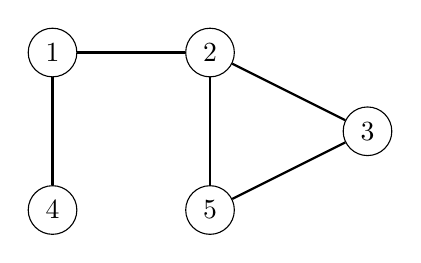
\begin{tikzpicture}
\node[draw, circle] (1) at (1,5) {$1$};
\node[draw, circle] (2) at (3,5) {$2$};
\node[draw, circle] (3) at (5,4) {$3$};
\node[draw, circle] (4) at (1,3) {$4$};
\node[draw, circle] (5) at (3,3) {$5$};

\path[draw,thick,-] (1) -- (2);
\path[draw,thick,-] (2) -- (3);
\path[draw,thick,-] (1) -- (4);
\path[draw,thick,-] (3) -- (5);
\path[draw,thick,-] (2) -- (5);
\end{tikzpicture}
\end{center}
Chúng ta có thể bắt đầu tìm kiếm tại bất kỳ nút nào của đồ thị;
bây giờ chúng ta sẽ bắt đầu tìm kiếm tại nút 1.

Tìm kiếm đầu tiên tiến đến nút 2:
\begin{center}
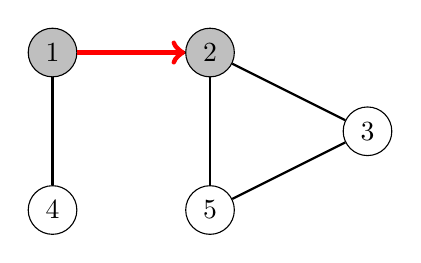
\begin{tikzpicture}
\node[draw, circle,fill=lightgray] (1) at (1,5) {$1$};
\node[draw, circle,fill=lightgray] (2) at (3,5) {$2$};
\node[draw, circle] (3) at (5,4) {$3$};
\node[draw, circle] (4) at (1,3) {$4$};
\node[draw, circle] (5) at (3,3) {$5$};

\path[draw,thick,-] (1) -- (2);
\path[draw,thick,-] (2) -- (3);
\path[draw,thick,-] (1) -- (4);
\path[draw,thick,-] (3) -- (5);
\path[draw,thick,-] (2) -- (5);

\path[draw=red,thick,->,line width=2pt] (1) -- (2);
\end{tikzpicture}
\end{center}
Sau đó, các nút 3 và 5 sẽ được duyệt:
\begin{center}
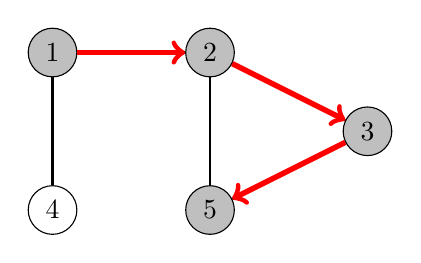
\begin{tikzpicture}
\node[draw, circle,fill=lightgray] (1) at (1,5) {$1$};
\node[draw, circle,fill=lightgray] (2) at (3,5) {$2$};
\node[draw, circle,fill=lightgray] (3) at (5,4) {$3$};
\node[draw, circle] (4) at (1,3) {$4$};
\node[draw, circle,fill=lightgray] (5) at (3,3) {$5$};

\path[draw,thick,-] (1) -- (2);
\path[draw,thick,-] (2) -- (3);
\path[draw,thick,-] (1) -- (4);
\path[draw,thick,-] (3) -- (5);
\path[draw,thick,-] (2) -- (5);

\path[draw=red,thick,->,line width=2pt] (1) -- (2);
\path[draw=red,thick,->,line width=2pt] (2) -- (3);
\path[draw=red,thick,->,line width=2pt] (3) -- (5);
\end{tikzpicture}
\end{center}
Các nút lân cận của nút 5 là 2 và 3,
nhưng tìm kiếm đã duyệt qua cả hai,
vì vậy đã đến lúc quay lại các nút trước đó.
Các nút lân cận của nút 3 và 2 cũng
đã được duyệt, vì vậy tiếp theo chúng ta di chuyển
từ nút 1 đến nút 4:
\begin{center}
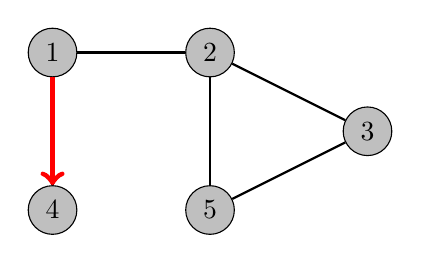
\begin{tikzpicture}
\node[draw, circle,fill=lightgray] (1) at (1,5) {$1$};
\node[draw, circle,fill=lightgray] (2) at (3,5) {$2$};
\node[draw, circle,fill=lightgray] (3) at (5,4) {$3$};
\node[draw, circle,fill=lightgray] (4) at (1,3) {$4$};
\node[draw, circle,fill=lightgray] (5) at (3,3) {$5$};

\path[draw,thick,-] (1) -- (2);
\path[draw,thick,-] (2) -- (3);
\path[draw,thick,-] (1) -- (4);
\path[draw,thick,-] (3) -- (5);
\path[draw,thick,-] (2) -- (5);

\path[draw=red,thick,->,line width=2pt] (1) -- (4);
\end{tikzpicture}
\end{center}
Sau đó, tìm kiếm kết thúc vì nó đã duyệt
tất cả các nút.

Độ phức tạp thời gian của tìm kiếm theo chiều sâu là $O(n+m)$
trong đó $n$ là số nút và $m$ là
số cạnh,
bởi vì thuật toán xử lý mỗi nút và cạnh một lần.

\subsubsection*{Cài đặt}

Tìm kiếm theo chiều sâu có thể được cài đặt
thuận tiện bằng cách sử dụng đệ quy.
Hàm \texttt{dfs} sau đây bắt đầu
một tìm kiếm theo chiều sâu tại một nút đã cho.
Hàm giả định rằng đồ thị được
lưu trữ dưới dạng danh sách kề trong một mảng
\begin{lstlisting}
vector<int> adj[N];
\end{lstlisting}
và cũng duy trì một mảng
\begin{lstlisting}
bool visited[N];
\end{lstlisting}
để theo dõi các nút đã được duyệt.
Ban đầu, mỗi giá trị mảng là \texttt{false},
và khi tìm kiếm đến nút $s$,
giá trị của \texttt{visited}[$s$] trở thành \texttt{true}.
Hàm có thể được cài đặt như sau:
\begin{lstlisting}
void dfs(int s) {
    if (visited[s]) return;
    visited[s] = true;
    // xu ly nut s
    for (auto u: adj[s]) {
        dfs(u);
    }
}
\end{lstlisting}

\section{Tìm kiếm theo chiều rộng}

\index{tìm kiếm theo chiều rộng}

\key{Tìm kiếm theo chiều rộng} (BFS) duyệt các nút
theo thứ tự tăng dần khoảng cách của chúng
từ nút bắt đầu.
Do đó, chúng ta có thể tính khoảng cách
từ nút bắt đầu đến tất cả các nút khác
bằng cách sử dụng tìm kiếm theo chiều rộng.
Tuy nhiên, tìm kiếm theo chiều rộng khó cài đặt hơn
so với tìm kiếm theo chiều sâu.

Tìm kiếm theo chiều rộng đi qua các nút
theo từng cấp độ một.
Đầu tiên, tìm kiếm khám phá các nút có
khoảng cách từ nút bắt đầu là 1,
sau đó là các nút có khoảng cách là 2, và cứ thế.
Quá trình này tiếp tục cho đến khi tất cả các nút
đã được duyệt.

\subsubsection*{Ví dụ}

Chúng ta hãy xem xét cách tìm kiếm theo chiều rộng xử lý
đồ thị sau:

\begin{center}
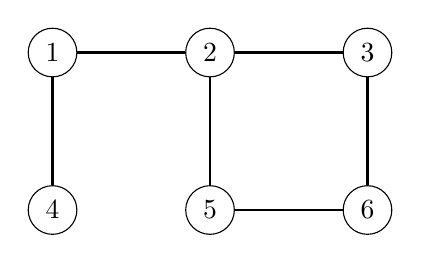
\begin{tikzpicture}
\node[draw, circle] (1) at (1,5) {$1$};
\node[draw, circle] (2) at (3,5) {$2$};
\node[draw, circle] (3) at (5,5) {$3$};
\node[draw, circle] (4) at (1,3) {$4$};
\node[draw, circle] (5) at (3,3) {$5$};
\node[draw, circle] (6) at (5,3) {$6$};

\path[draw,thick,-] (1) -- (2);
\path[draw,thick,-] (2) -- (3);
\path[draw,thick,-] (1) -- (4);
\path[draw,thick,-] (3) -- (6);
\path[draw,thick,-] (2) -- (5);
\path[draw,thick,-] (5) -- (6);
\end{tikzpicture}
\end{center}
Giả sử rằng tìm kiếm bắt đầu tại nút 1.
Đầu tiên, chúng ta xử lý tất cả các nút có thể đến được
từ nút 1 bằng một cạnh duy nhất:
\begin{center}
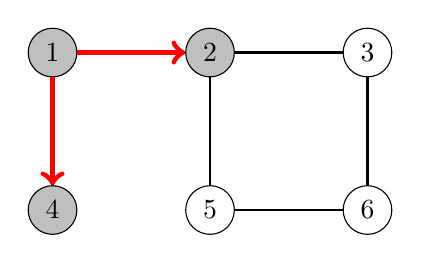
\begin{tikzpicture}
\node[draw, circle,fill=lightgray] (1) at (1,5) {$1$};
\node[draw, circle,fill=lightgray] (2) at (3,5) {$2$};
\node[draw, circle] (3) at (5,5) {$3$};
\node[draw, circle,fill=lightgray] (4) at (1,3) {$4$};
\node[draw, circle] (5) at (3,3) {$5$};
\node[draw, circle] (6) at (5,3) {$6$};

\path[draw,thick,-] (1) -- (2);
\path[draw,thick,-] (2) -- (3);
\path[draw,thick,-] (1) -- (4);
\path[draw,thick,-] (3) -- (6);
\path[draw,thick,-] (2) -- (5);
\path[draw,thick,-] (5) -- (6);

\path[draw,thick,-] (1) -- (2);
\path[draw,thick,-] (2) -- (3);
\path[draw,thick,-] (1) -- (4);
\path[draw,thick,-] (2) -- (5);

\path[draw=red,thick,->,line width=2pt] (1) -- (2);
\path[draw=red,thick,->,line width=2pt] (1) -- (4);
\end{tikzpicture}
\end{center}
Sau đó, chúng ta tiếp tục đến các nút 3 và 5:
\begin{center}
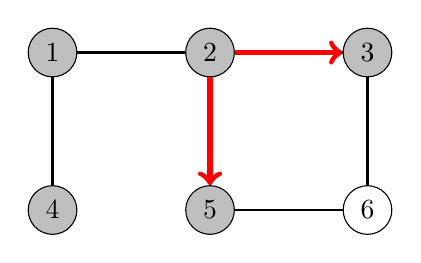
\begin{tikzpicture}
\node[draw, circle,fill=lightgray] (1) at (1,5) {$1$};
\node[draw, circle,fill=lightgray] (2) at (3,5) {$2$};
\node[draw, circle,fill=lightgray] (3) at (5,5) {$3$};
\node[draw, circle,fill=lightgray] (4) at (1,3) {$4$};
\node[draw, circle,fill=lightgray] (5) at (3,3) {$5$};
\node[draw, circle] (6) at (5,3) {$6$};

\path[draw,thick,-] (1) -- (2);
\path[draw,thick,-] (2) -- (3);
\path[draw,thick,-] (1) -- (4);
\path[draw,thick,-] (3) -- (6);
\path[draw,thick,-] (2) -- (5);
\path[draw,thick,-] (5) -- (6);

\path[draw,thick,-] (1) -- (2);
\path[draw,thick,-] (2) -- (3);
\path[draw,thick,-] (1) -- (4);
\path[draw,thick,-] (2) -- (5);

\path[draw=red,thick,->,line width=2pt] (2) -- (3);
\path[draw=red,thick,->,line width=2pt] (2) -- (5);
\end{tikzpicture}
\end{center}
Cuối cùng, chúng ta duyệt nút 6:
\begin{center}
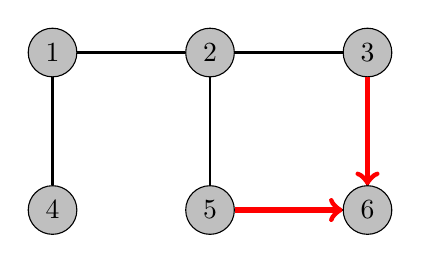
\begin{tikzpicture}
\node[draw, circle,fill=lightgray] (1) at (1,5) {$1$};
\node[draw, circle,fill=lightgray] (2) at (3,5) {$2$};
\node[draw, circle,fill=lightgray] (3) at (5,5) {$3$};
\node[draw, circle,fill=lightgray] (4) at (1,3) {$4$};
\node[draw, circle,fill=lightgray] (5) at (3,3) {$5$};
\node[draw, circle,fill=lightgray] (6) at (5,3) {$6$};

\path[draw,thick,-] (1) -- (2);
\path[draw,thick,-] (2) -- (3);
\path[draw,thick,-] (1) -- (4);
\path[draw,thick,-] (3) -- (6);
\path[draw,thick,-] (2) -- (5);
\path[draw,thick,-] (5) -- (6);

\path[draw,thick,-] (1) -- (2);
\path[draw,thick,-] (2) -- (3);
\path[draw,thick,-] (1) -- (4);
\path[draw,thick,-] (2) -- (5);

\path[draw=red,thick,->,line width=2pt] (3) -- (6);
\path[draw=red,thick,->,line width=2pt] (5) -- (6);
\end{tikzpicture}
\end{center}
Bây giờ chúng ta đã tính được khoảng cách
từ nút bắt đầu đến tất cả các nút của đồ thị.
Các khoảng cách như sau:

\begin{tabular}{ll}
\\
nút & khoảng cách \\
\hline
1 & 0 \\
2 & 1 \\
3 & 2 \\
4 & 1 \\
5 & 2 \\
6 & 3 \\
\\
\end{tabular}

Giống như trong tìm kiếm theo chiều sâu,
độ phức tạp thời gian của tìm kiếm theo chiều rộng
là $O(n+m)$, trong đó $n$ là số nút
và $m$ là số cạnh.

\subsubsection*{Cài đặt}

Tìm kiếm theo chiều rộng khó cài đặt hơn
so với tìm kiếm theo chiều sâu,
bởi vì thuật toán duyệt các nút
ở các phần khác nhau của đồ thị.
Một cài đặt điển hình dựa trên
một hàng đợi chứa các nút.
Tại mỗi bước, nút tiếp theo trong hàng đợi
sẽ được xử lý.

Đoạn mã sau giả định rằng đồ thị được lưu trữ
dưới dạng danh sách kề và duy trì các
cấu trúc dữ liệu sau:
\begin{lstlisting}
queue<int> q;
bool visited[N];
int distance[N];
\end{lstlisting}

Hàng đợi \texttt{q}
chứa các nút cần được xử lý
theo thứ tự tăng dần khoảng cách của chúng.
Các nút mới luôn được thêm vào cuối
hàng đợi, và nút ở đầu
hàng đợi là nút tiếp theo cần được xử lý.
Mảng \texttt{visited} chỉ ra
những nút nào mà tìm kiếm đã duyệt qua,
và mảng \texttt{distance} sẽ chứa
khoảng cách từ nút bắt đầu đến tất cả các nút của đồ thị.

Tìm kiếm có thể được cài đặt như sau,
bắt đầu tại nút $x$:
\begin{lstlisting}
visited[x] = true;
distance[x] = 0;
q.push(x);
while (!q.empty()) {
    int s = q.front(); q.pop();
    // xu ly nut s
    for (auto u : adj[s]) {
        if (visited[u]) continue;
        visited[u] = true;
        distance[u] = distance[s]+1;
        q.push(u);
    }
}
\end{lstlisting}

\section{Ứng dụng}

Sử dụng các thuật toán duyệt đồ thị,
chúng ta có thể kiểm tra nhiều thuộc tính của đồ thị.
Thông thường, cả tìm kiếm theo chiều sâu và
tìm kiếm theo chiều rộng đều có thể được sử dụng,
nhưng trong thực tế, tìm kiếm theo chiều sâu
là một lựa chọn tốt hơn, vì nó
dễ cài đặt hơn.
Trong các ứng dụng sau, chúng ta sẽ
giả định rằng đồ thị là vô hướng.

\subsubsection{Kiểm tra tính liên thông}

\index{đồ thị liên thông}

Một đồ thị là liên thông nếu có một đường đi
giữa hai nút bất kỳ của đồ thị.
Do đó, chúng ta có thể kiểm tra xem một đồ thị có liên thông hay không
bằng cách bắt đầu tại một nút tùy ý và
tìm hiểu xem chúng ta có thể đến được tất cả các nút khác hay không.

Ví dụ, trong đồ thị
\begin{center}
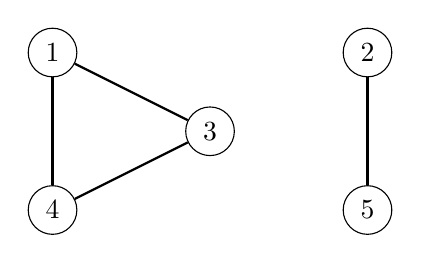
\begin{tikzpicture}
\node[draw, circle] (2) at (7,5) {$2$};
\node[draw, circle] (1) at (3,5) {$1$};
\node[draw, circle] (3) at (5,4) {$3$};
\node[draw, circle] (5) at (7,3) {$5$};
\node[draw, circle] (4) at (3,3) {$4$};

\path[draw,thick,-] (1) -- (3);
\path[draw,thick,-] (1) -- (4);
\path[draw,thick,-] (3) -- (4);
\path[draw,thick,-] (2) -- (5);
\end{tikzpicture}
\end{center}
một tìm kiếm theo chiều sâu từ nút $1$ duyệt
các nút sau:
\begin{center}
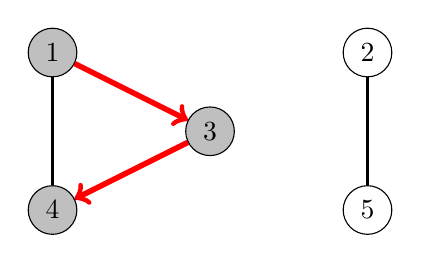
\begin{tikzpicture}
\node[draw, circle] (2) at (7,5) {$2$};
\node[draw, circle,fill=lightgray] (1) at (3,5) {$1$};
\node[draw, circle,fill=lightgray] (3) at (5,4) {$3$};
\node[draw, circle] (5) at (7,3) {$5$};
\node[draw, circle,fill=lightgray] (4) at (3,3) {$4$};

\path[draw,thick,-] (1) -- (3);
\path[draw,thick,-] (1) -- (4);
\path[draw,thick,-] (3) -- (4);
\path[draw,thick,-] (2) -- (5);

\path[draw=red,thick,->,line width=2pt] (1) -- (3);
\path[draw=red,thick,->,line width=2pt] (3) -- (4);

\end{tikzpicture}
\end{center}

Vì tìm kiếm không duyệt qua tất cả các nút,
chúng ta có thể kết luận rằng đồ thị không liên thông.
Tương tự, chúng ta cũng có thể tìm thấy tất cả các thành phần liên thông
của một đồ thị bằng cách lặp qua các nút và luôn
bắt đầu một tìm kiếm theo chiều sâu mới nếu nút hiện tại
chưa thuộc về bất kỳ thành phần nào.

\subsubsection{Tìm chu trình}

\index{chu trình}

Một đồ thị chứa một chu trình nếu trong quá trình duyệt đồ thị,
chúng ta tìm thấy một nút có hàng xóm (khác với
nút trước đó trong đường đi hiện tại) đã được
duyệt.
Ví dụ, đồ thị
\begin{center}
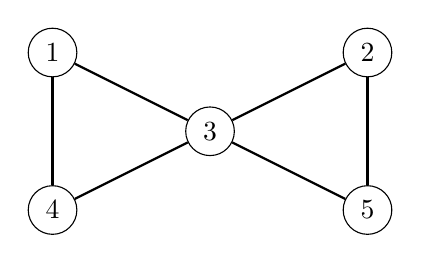
\begin{tikzpicture}
\node[draw, circle] (2) at (7,5) {$2$};
\node[draw, circle] (1) at (3,5) {$1$};
\node[draw, circle] (3) at (5,4) {$3$};
\node[draw, circle] (5) at (7,3) {$5$};
\node[draw, circle] (4) at (3,3) {$4$};

\path[draw,thick,-] (1) -- (3);
\path[draw,thick,-] (1) -- (4);
\path[draw,thick,-] (3) -- (4);
\path[draw,thick,-] (2) -- (5);
\path[draw,thick,-] (2) -- (3);
\path[draw,thick,-] (3) -- (5);
\end{tikzpicture}
\end{center}
chứa hai chu trình và chúng ta có thể tìm thấy một
trong số chúng như sau:
\begin{center}
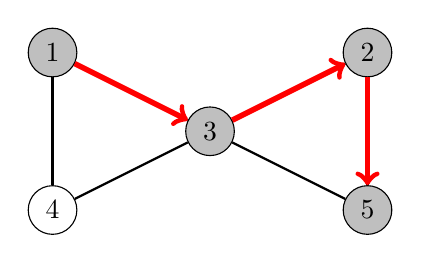
\begin{tikzpicture}
\node[draw, circle,fill=lightgray] (2) at (7,5) {$2$};
\node[draw, circle,fill=lightgray] (1) at (3,5) {$1$};
\node[draw, circle,fill=lightgray] (3) at (5,4) {$3$};
\node[draw, circle,fill=lightgray] (5) at (7,3) {$5$};
\node[draw, circle] (4) at (3,3) {$4$};

\path[draw,thick,-] (1) -- (3);
\path[draw,thick,-] (1) -- (4);
\path[draw,thick,-] (3) -- (4);
\path[draw,thick,-] (2) -- (5);
\path[draw,thick,-] (2) -- (3);
\path[draw,thick,-] (3) -- (5);

\path[draw=red,thick,->,line width=2pt] (1) -- (3);
\path[draw=red,thick,->,line width=2pt] (3) -- (2);
\path[draw=red,thick,->,line width=2pt] (2) -- (5);

\end{tikzpicture}
\end{center}
Sau khi di chuyển từ nút 2 đến nút 5, chúng ta nhận thấy rằng
hàng xóm 3 của nút 5 đã được duyệt.
Do đó, đồ thị chứa một chu trình đi qua nút 3,
ví dụ, $3 \rightarrow 2 \rightarrow 5 \rightarrow 3$.

Một cách khác để tìm hiểu xem một đồ thị có chứa chu trình hay không
là chỉ cần tính số lượng nút và cạnh
trong mọi thành phần.
Nếu một thành phần chứa $c$ nút và không có chu trình,
nó phải chứa chính xác $c-1$ cạnh
(vì vậy nó phải là một cây).
Nếu có $c$ hoặc nhiều cạnh hơn, thành phần đó
chắc chắn chứa một chu trình.

\subsubsection{Kiểm tra tính hai phía}

\index{đồ thị hai phía}

Một đồ thị là hai phía nếu các nút của nó có thể được tô màu
bằng hai màu sao cho không có các
nút kề nhau nào có cùng màu.
Thật đáng ngạc nhiên là dễ dàng kiểm tra xem một đồ thị
có phải là hai phía hay không bằng cách sử dụng các thuật toán duyệt đồ thị.

Ý tưởng là tô màu nút bắt đầu màu xanh,
tất cả các hàng xóm của nó màu đỏ, tất cả các hàng xóm của chúng màu xanh, và cứ thế.
Nếu tại một thời điểm nào đó của tìm kiếm, chúng ta nhận thấy rằng
hai nút kề nhau có cùng màu,
điều này có nghĩa là đồ thị không phải là hai phía.
Ngược lại, đồ thị là hai phía và một cách tô màu
đã được tìm thấy.

Ví dụ, đồ thị
\begin{center}
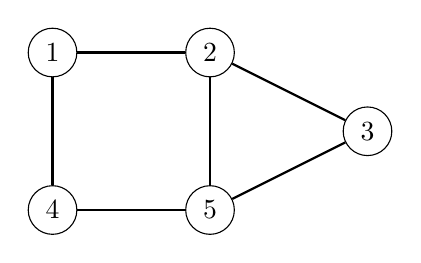
\begin{tikzpicture}
\node[draw, circle] (2) at (5,5) {$2$};
\node[draw, circle] (1) at (3,5) {$1$};
\node[draw, circle] (3) at (7,4) {$3$};
\node[draw, circle] (5) at (5,3) {$5$};
\node[draw, circle] (4) at (3,3) {$4$};

\path[draw,thick,-] (1) -- (2);
\path[draw,thick,-] (2) -- (5);
\path[draw,thick,-] (5) -- (4);
\path[draw,thick,-] (4) -- (1);
\path[draw,thick,-] (2) -- (3);
\path[draw,thick,-] (5) -- (3);
\end{tikzpicture}
\end{center}
không phải là hai phía, bởi vì một tìm kiếm từ nút 1
tiến hành như sau:
\begin{center}
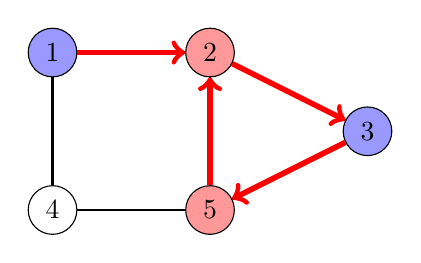
\begin{tikzpicture}
\node[draw, circle,fill=red!40] (2) at (5,5) {$2$};
\node[draw, circle,fill=blue!40] (1) at (3,5) {$1$};
\node[draw, circle,fill=blue!40] (3) at (7,4) {$3$};
\node[draw, circle,fill=red!40] (5) at (5,3) {$5$};
\node[draw, circle] (4) at (3,3) {$4$};

\path[draw,thick,-] (1) -- (2);
\path[draw,thick,-] (2) -- (5);
\path[draw,thick,-] (5) -- (4);
\path[draw,thick,-] (4) -- (1);
\path[draw,thick,-] (2) -- (3);
\path[draw,thick,-] (5) -- (3);

\path[draw=red,thick,->,line width=2pt] (1) -- (2);
\path[draw=red,thick,->,line width=2pt] (2) -- (3);
\path[draw=red,thick,->,line width=2pt] (3) -- (5);
\path[draw=red,thick,->,line width=2pt] (5) -- (2);
\end{tikzpicture}
\end{center}
Chúng ta nhận thấy rằng màu của cả hai nút 2 và 5
là màu đỏ, trong khi chúng là các nút kề nhau trong đồ thị.
Do đó, đồ thị không phải là hai phía.

Thuật toán này luôn hoạt động, bởi vì khi chỉ
có hai màu có sẵn,
màu của nút bắt đầu trong một thành phần
xác định màu của tất cả các nút khác trong thành phần đó.
Không có sự khác biệt nào cho dù
nút bắt đầu là màu đỏ hay màu xanh.

Lưu ý rằng trong trường hợp tổng quát,
rất khó để tìm ra liệu các nút
trong một đồ thị có thể được tô màu bằng $k$ màu
sao cho không có nút kề nhau nào có cùng màu hay không.
Ngay cả khi $k=3$, không có thuật toán hiệu quả nào được biết đến
mà vấn đề là NP-khó.
